\documentclass[a4paper,12pt,final]{article}


\usepackage{graphicx}
\title{
\begin{center}
  	
\includegraphics[scale=0.3]{101Logo.png} 
  \end{center}
  \textbf{\\}
CSIR - Distributed Application Manager\\
Architectural Requirements Document\\
}
\author{101 Solutions}
\begin{document}
\maketitle
\thispagestyle{empty}
\newpage
\tableofcontents
\thispagestyle{empty}
\newpage
Change Log
\vspace{6pt}\newline
\begin{tabular}{|l|l|l|}
\hline
Date & Version & Description\\
\hline
13 Jul & Version 0.1 & Document Created\\
\hline
23 Jul & Version 0.2 & Added section 1.4 and 4\\
\hline
25 Jul & Version 0.3 & Added versioning system\\
\hline
25 Jul & Version 0.4 & Added initial section 2 and 6\\
\hline
26 Jul & Version 0.5 & Completed section 1.2\\
\hline
27 Jul & Version 0.6 & Completed section 3\\
\hline
28 Jul & Version 0.7 & Completed section 1.3 and 5\\
\hline
28 Jul & Version 0.8 & Proofread and added some content\\
\hline
28 Jul & Version 0.9 & Added glossary section\\
\hline
\end{tabular}

\pagenumbering{arabic}
\section{Architecture requirements}
\subsection{Architectural scope}
\begin{itemize}
\item Providing infrastructure for copying, synchronizing and managinge files over multiple computers from one master
\item Provide infrastructure supporting communication between more than one computer
\item Providing 
\end{itemize}
\subsection{Quality requirements}
The following Quality requirements will be implemented in the system:
\begin{itemize}
\item \textbf{Installability} - The software should be able to easily install on any of the required platforms, without the need for further adjustments or 3rd party applications.
\item \textbf{Performance} - The software should be able to run optimally. Specifically when copying required build files, for example one large file will copy faster than many small files.
\item \textbf{Usability} - The software should be easy to use without the need to read extensive documentation on how to operate it.
\item \textbf{Look and feel} - Look and feel ties in with usabilty.  How the software looks should conform to how it will be used, which should be in a visually intuitive manner.
\item \textbf{Reusability} - The software should be able to be reused within different contexts, while still fulfilling the necessary functional requirements.
\item \textbf{Reliability} - The software should be reliable in the sense that especially when build versions are updated that all the required files are sent and recieved without failures.
\end{itemize}
\subsection{Integration and access channel requirements}
Our system can interact with Subversion (SVN), which is where the clients store the various builds of their applications. We will also be connecting to a MySql database where the information concerning confiugurations on slave pc's will be stored. XML is also an option for storing information.
\begin{itemize}
\item We can use the SVN client library to connesct to Subversion.
\item Connector/C++ 1.1.3 is available to connect to MySql for both Windows and Linux.
\item XML parsing and handling is supported through SAX and DOM compliant APIs as well as streaming classes in Qt.
\end{itemize}
The system will be accessible to users via a Graphical User Interface as specified by the client.
\subsection{Architectural constraints}
Overall constraints include the use of QT 4.8.4 with C++ throughout the project. The use of other technologies are allowed if need be such as 7zip for zipping of files and unzipping of files, however it would be advisable to use a QT API such as the file handling API to do so. Furthermore the project must be deployable on windows and linux and be capable of working on each of them.
\vspace{6pt}\newline
For phase 2 in the project, the project must be capable of running applications on the slave computers that have been distributed from a master computer to a slave. The configuration for the application to be run should also be used when running the program so that different environments can be selected.

\section{Architectural patterns or styles}
The project will make use of a Layered system combined with a Client server architecture. The project  needs the division of functionality for copying files, network, database and other.
\vspace{6pt}\newline
%Section Describing the layered system integrated in program
\subsection{Layered system}
\begin{tabular}{|l|l|p{8cm}|}   
\hline
Layer Number & Name & Description\\
\hline
5 & GUI & Displays all the func\\
\hline
4 & Management & A management facade to combine functionality of other layers\\
\hline
3 & Database & A layer that will manage the information of the builds(applications)\\
\hline
1 & Networking & The layer with services to connect and speak to other computers\\
\hline
\end{tabular}

%Section describing the 
\subsection{Client server}
Client can in this case be the Master Computer or the Slave Computer. The server could potentially be in the Master or in the Slave, depending on the situation.
\begin{center}
  	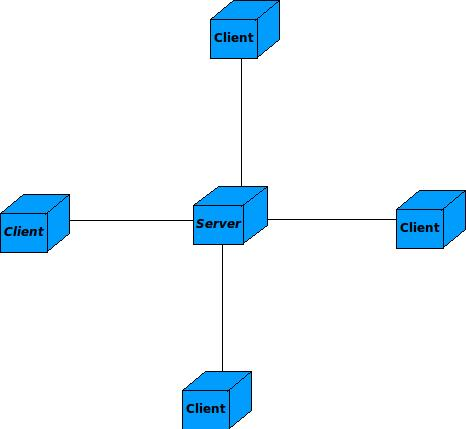
\includegraphics[scale=0.6]{ClientServer.jpeg} 
  \end{center}

\section{Architectural tactics or strategies}
For each quality requirements the following tactics will be used as a guide to solve them:
\begin{itemize}
\item \textbf{Installability} - Using the QT framework, which allows source code to be built for various platforms, the software should be able to install and work on those platforms.
\item \textbf{Performance} - Compiling and copying larger files will be quicker than copying a lot of small files. Using 7zip to compress small files will increase performance.
\item \textbf{Usability} - Using simple design and tooltips will allow for easy understanding of how the software is supposed to be used.  A quick help section will also enhance understanding and usability.
\item \textbf{Look and feel} - Usabilty should also be enhanced by a visual intuitive layout that makes sense, is very simple and does not require typing.  A simple drag and drop feature will be used to achieve this.
\item \textbf{Reusability} - The saving of configuations will allow the software to easily be reused to recreate simulations that have been run before.
\item \textbf{Reliability} - Using coding protocols that will check that a message was successfully sent and received, such as TCP, will ensure a reliable connection.
\end{itemize}

\section{Use of reference architectures and\\ frameworks}
QT is a framework much the same as Java and their motto stated "Code Less. Create More. Deploy Everywhere." which means the framework allows cross platform development and deployment. This project will make use of QT 4.8.4 framework with C++ that will enable the project to be used on multiple platforms. We will strive to make use of the QT API's to provide a project with capabilities of compiling and running on multiple platforms.
\vspace{6pt}\newline
QT 4.8.4 contains file API's such as QFile and QFileSystemWatcher and QDirIterator which can be used for synchronization of files and folders accross multiple computers. QFile will help with writing and editing of files that may be used in this project. The QFileSystemWatcher can be used to monitor a directory structure that may be specified by a user and if changes occur the changes can then be spread accross to the slave computers. The QDirIterator can be used to manipulate folders and directories if need be.
\vspace{6pt}\newline
QT also contains an extensive API for networking that we can make use of when implementing the project. This will allow the slave and master computers to communicate and transfer files from one computer to the other. The applications can be run on multiple slaves by making use of QT networking capabilities. Examples of those networking API's are QUdpSocket and QTcpSocket that can be used to create connections between computers. The QNetworkInterface class can be used to obtain information on networking interfaces that a computer has if the need arises.
\section{Access and integration channels}
Below is a rough depiction of how the GUI will look. The different nodes each have a colour to indicate status. Green means ready, Yellow means some error has occured, Red means it is offline. A program build can be clicked on the list and placed on the slave it is needed on. This will initiate the copying sequence. Next a simulation is chosen and can be run.\\
\begin{center}
  	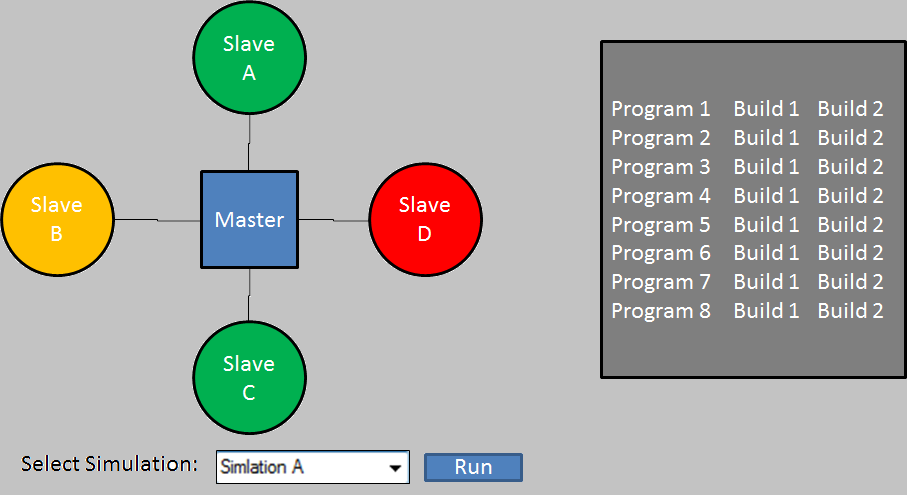
\includegraphics[scale=0.65]{GuiPlan.png} 
  \end{center}
Below are the various channels we will be using:
\begin{itemize}
\item We can use the SVN client library to connect to Subversion. Subversion has a modular design: it's implemented as a collection of libraries written in C. Each library has a well-defined purpose and API, and that interface is available not only for Subversion itself to use, but for any software that wishes to embed or otherwise programmatically control Subversion. Additionally, Subversion's API is available not only to other C programs, but also to programs written in higher-level languages such as Python, Perl, Java, and Ruby.
\item Connector/C++ 1.1.3 is available to connect to MySql for both Windows and Linux. It is a MySQL database connector for C++. It lets you develop C++ applications that connect to the MySQL Server.
\item XML parsing and handling is supported through SAX and DOM compliant APIs as well as streaming classes in Qt. Additionally the QtXmlPatterns modules provide classes for querying XML files and custom data models.
\end{itemize}
\section{Technologies}

\begin{itemize}

\item{Platforms}
\begin{itemize}
\item{Windows}
\item{Linux}
\end{itemize}


\item{Database}
\begin{itemize}
\item{XML based or}
\item{MySQL based}
\end{itemize}


\item{Network}
\begin{itemize}
\item{QT Framework Network API}
\end{itemize}


\item{Graphical user interface}
\begin{itemize}
\item{QT Framework GUI API}
\end{itemize}

\end{itemize}


\section{Glossary}
\begin{itemize}
\item{Build - An application build version that could potentially be distrobuted to slave computers}
\item{Slave - A computer that will be controlled via a master computer. Application builds will be sent to this computer.}
\item{Master - A computer that will control Slaves across a network}
\item{Server - A machine waiting on the network for connections from other machines}
\item{GUI - Graphical user interface with which a user can control the project}
\item{Project - This project. The distrobuted application manager}
\item{Application Configuration - Environment variables that are specified when running an application}
\end{itemize}

\end{document}